% !TEX root = ../main.tex

\section{Introduction}



Ethereum is an public blockchain proposed in 2013, deployed in 2015~\cite{Ref00}, and has the second largest market cap at the time of writing\footnote{CoinMarketCap - Ethereum currency - Accessed: 2019-02-11 \newline\url{https://coinmarketcap.com/currencies/ethereum/}}. It has a large development community which track enhancements and propose new ideas.\footnote{CoinDesk Crypto-Economics Explorer - Accessed: 2019-02-11 \newline\url{https://www.coindesk.com/data}} Ethereum enables decentralized applications (\dapps) to be deployed and executed. DApps can accept and transfer Ethereum's built-in currency (ETH) or might issue their own custom currency-like tokens for specific purposes.

Tokens might be currencies with different properties than ETH, they may be tokens that are required for access to a DApp's functionality or they might represent ownership of some off-blockchain asset. It is beneficial to have interoperable tokens with other DApps and off-blockchain webapps, such as exchange services that allow tokens to be traded. Toward this goal, the Ethereum project accepted a proposed standard (called ERC20~\cite{Ref08}) for a set of methods which standard-compliant tokens should implement. In terms of object oriented programming, ERC20 is an interface that defines abstract methods (name, parameters, return types) and provides guidelines on how the methods should be implemented, however it does not provide a actual concrete implementation (see Figure~\ref{fig:erc20api}). 

\begin{figure}[t!]
	\centering
	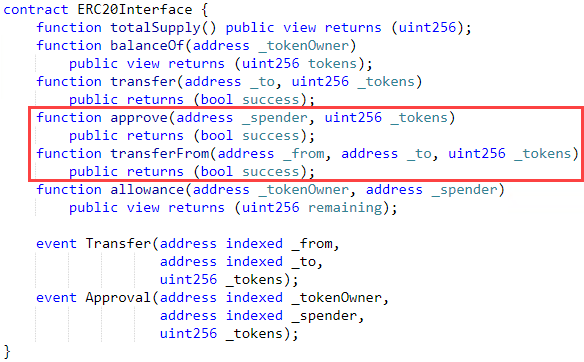
\includegraphics[width=1.0\linewidth]{figures/multiple_withdrawal_01.png}
	\caption{ERC20 API defines 6 functions and 2 events that have to be implemented as part of ERC20-compliant token. Using \texttt{approve()} and \texttt{transferFrom} functions in existence of race condition may lead to \textit{``multiple withdrawal attack''}\label{fig:erc20api}}
\end{figure}

% the blockchain. Tokens are essential part of this ecosystem which define set of rules---known as API\footnote{Advanced Programming Interface.}---for standardizing interaction with smart contracts.\footnote{Types of transactions that execute as they are programmed by Ethereum scripting language (e.g., Solidity or Vyper)}. Therefore, any ERC20\footnote{ERC20 is title of the standard and it should be referred as EIP20 (which is the actual proposal for improvement). In this paper we use both ERC20 and EIP20 in one sense for simplicity.}-compliant application can interact with any ERC20 token for trading, swapping, exchanging, etc. For example, shares of company X can be represented as ERC20 tokens to be reusable by other smart contracts (e.g., online exchanges, automated payment systems, decentralized games, etc). Leveraging ERC20 token facilitates implementation of financial assets while raising some security concerns. ERC20 tokens are technically standardized version of smart contracts that could be similarly vulnerable to security flaws.

% Jeremy: This seems unnecessary:
%\begin{figure}[t]
%	\centering
%	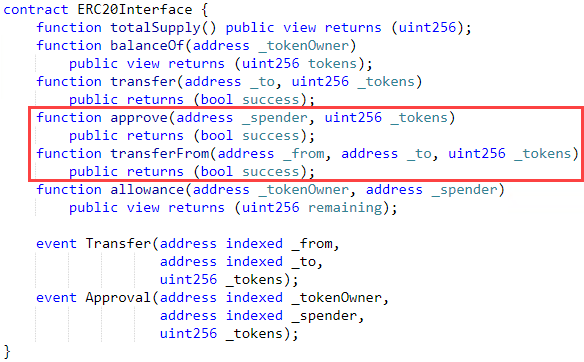
\includegraphics[width=1.0\linewidth]{figures/multiple_withdrawal_01.png}
%	\caption{Importance of ERC20 security in case of (1) digitizing share of company X (2) representing a fiat currency. In this case, smart contracts interact with two different ERC20 tokens which are repressing in sequence, a financial instrument and a non-collateralized stablecoin. Any security vulnerability in written code of ERC20 tokens, will impact security of related smart contracts and value of underlying assets.}
%\end{figure}

Since introduction of ERC20 API in November 2015, several vulnerabilities have been discovered and addressed. In October 2017, a security issue called \textit{``Multiple Withdrawal Attack''} was opened on GitHub\cite{Ref13,Ref07}. The attack originates from two methods in the ERC20 standard for approving and transferring tokens. The use of these functions in an undesirable situation (\eg front-running~\cite{eskandari2019sok}) could result in more tokens being spent by the allowed third party. This issue is still open and several solutions have been made to mitigate it. We started off by analyzing two implementations of ERC20 token provided by OpenZeppelin\cite{Ref10} and ConsenSys\cite{Ref11}. They advised by authors of ERC20 standard \cite{Ref08} as sample. OpenZeppelin implementation mitigates the attack by introducing two additional methods as replacement of \texttt{approve()} method and ConsenSys implementation does not attempt to resolve the attack. Other implementations have a variety of different trade-offs in solving the issue which will be discussed separately.

\subsubsection*{Contributions} In this paper, we discuss 10 proposed solutions to the attack and evaluate them according to set of criteria that we developed in terms of compatibility with the standard and attack mitigation (see the summary in Figure~\ref{tab:comp}). Since none of them precisely satisfy constraints of ERC20 standard, we were motivated to propose new solutions to mitigate the attack. Specifically, we propose two new approaches: each secures one of the two vulnerable methods (\ie \texttt{approve} or \texttt{transferFrom}). The first one, mitigates the attack by comparing transferred tokens with the current allowance in the \texttt{approve} method. It uses \textit{Compare and Set (CAS)} pattern\cite{Ref06} to cover gap between transactions as root cause of the attack. CAS is one of the most widely used lock-free synchronization strategy that allows comparing and setting values in an atomic way. By leveraging this pattern, the gap between transactions will be removed and there is no possibility of effecting the attack. We would consider this solution as partially ERC20-compliant solution since it violates one of ERC20 constraints that prohibits any adjustment in the allowance. As we discuss further, it would not be feasible to secure \texttt{approve} method without adjusting allowance. Alternatively, securing \texttt{transferFrom} method has been considered as effective solution by not allowing token transfers more than allowed.

\begin{figure}[t!]
	\centering
	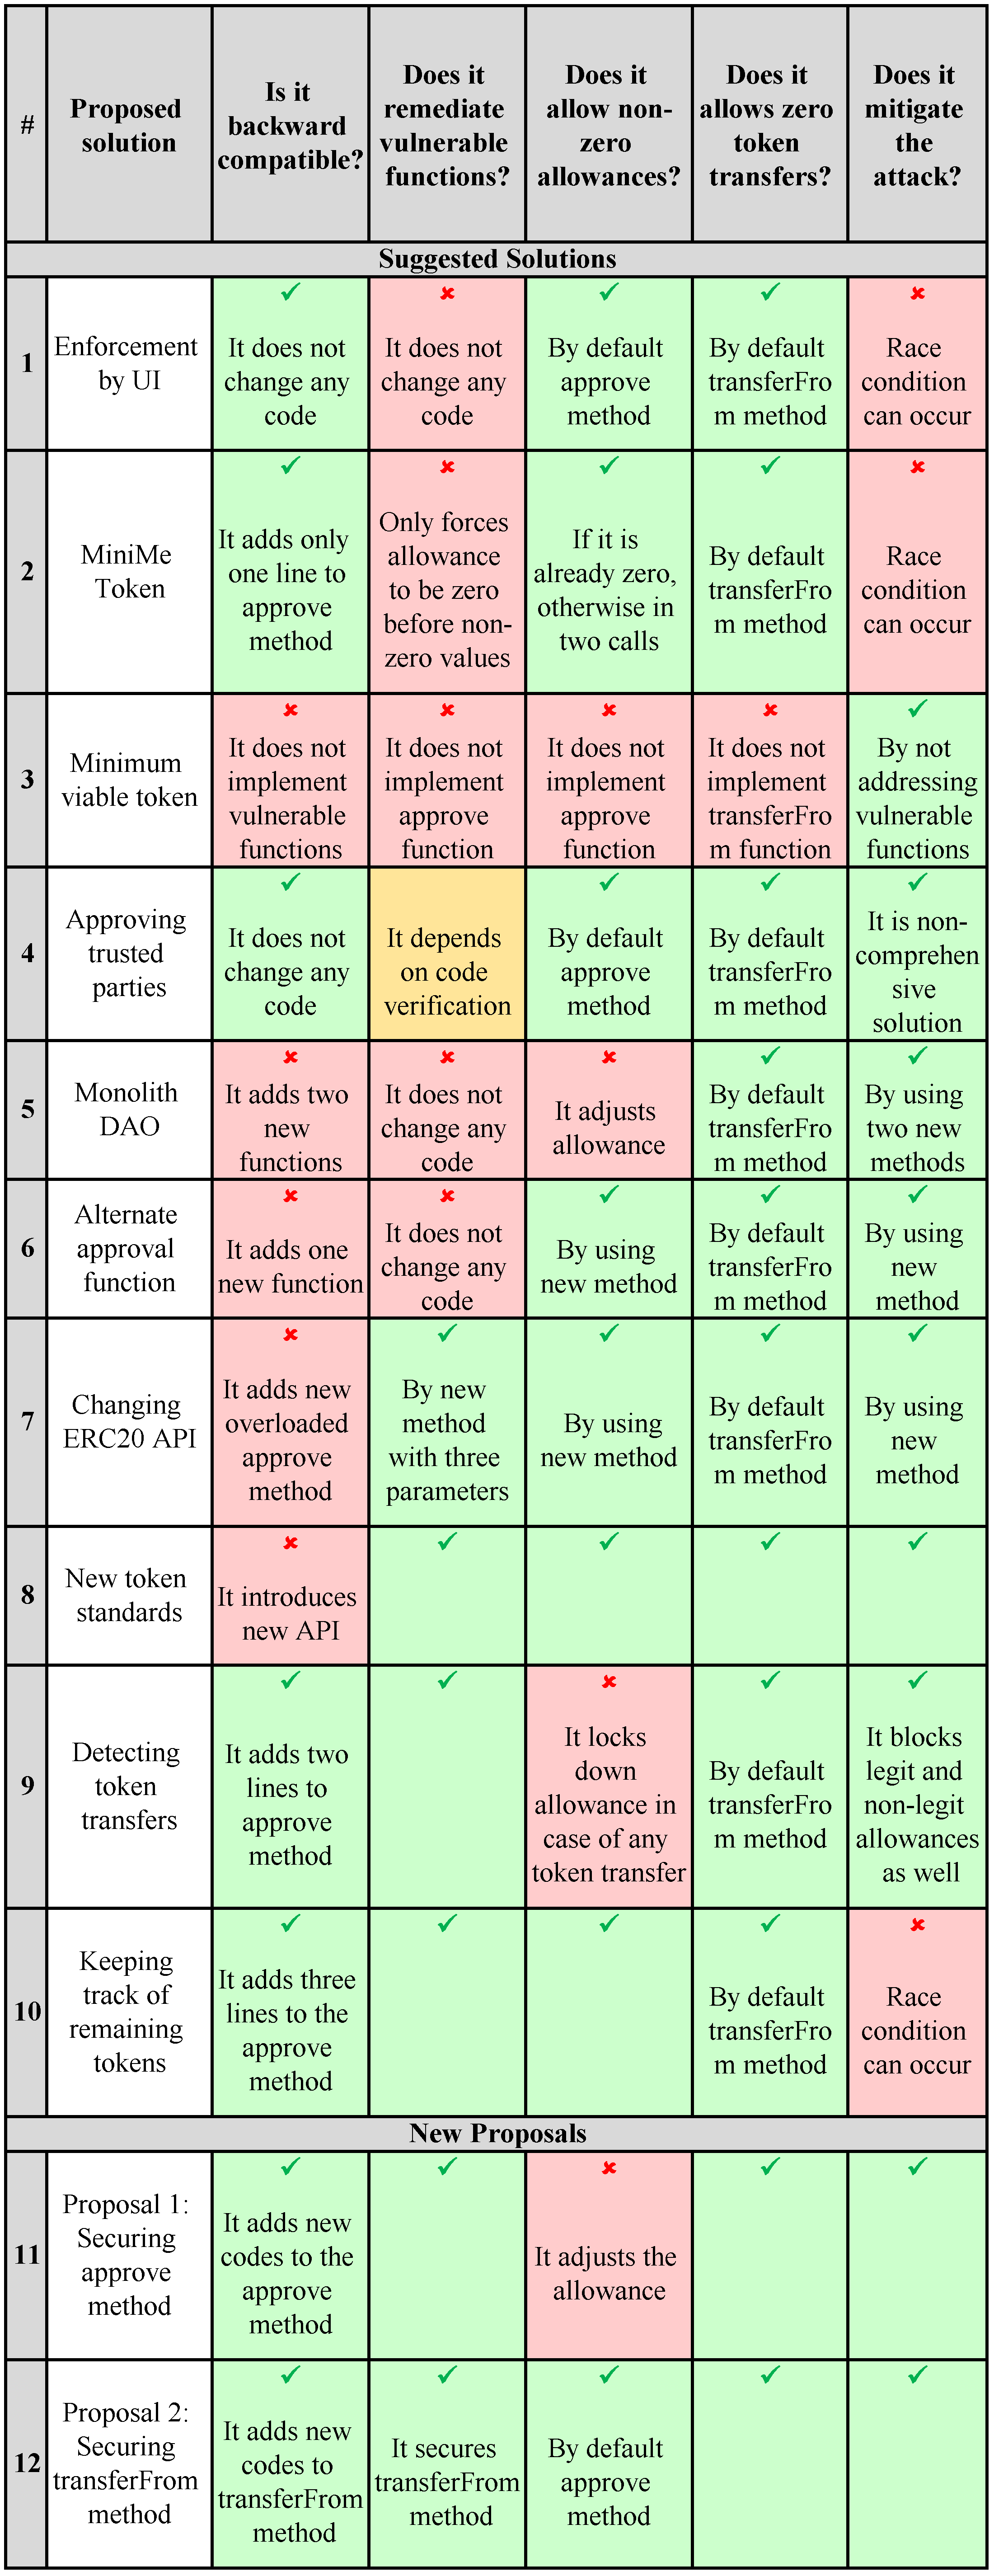
\includegraphics[width=1.0\linewidth]{figures/multiple_withdrawal_34.png}
	\caption{Comparison of 10 suggested solutions with two proposals contributed by this paper. In proposal 1, CAS pattern is used to mitigate the attack by comparing transferred tokens with new allowance. It is not ERC20-compliance since it adjusts the allowance. In proposal 2, a new local variable has been defined to keep tracking of transferred tokens and prevent more transfers in case of already transferred tokens. It secures \texttt{transferFrom} function and prevent the attack sustainably.\label{tab:comp}}
\end{figure}
